\documentclass{article}

% ==================== NeurIPS 2026 Template Settings ====================
% Download neurips_2026.sty from the NeurIPS submission page and place in same dir
\usepackage[final]{neurips_2026}

% ==================== Packages ====================
\usepackage[utf8]{inputenc}
\usepackage[T1]{fontenc}
\usepackage{hyperref}
\usepackage{url}
\usepackage{booktabs}
\usepackage{amsfonts, amsmath, amssymb}
\usepackage{graphicx}
\usepackage{subcaption}
\usepackage{algorithm}
\usepackage{algorithmic}
\usepackage{multirow}
\usepackage{xcolor}

% ==================== Title ====================
\title{AI4AI-Bench: Auditing Recursive Self-Improvement in LLM Agents}

\author{
  Anonymous Author(s) \\
  Affiliation \\
  \texttt{email@example.com}
}

% If the draft option is enabled, missing figures compile as placeholder boxes.
\usepackage{ifdraft}

\begin{document}

\maketitle

\begin{abstract}
Large language model agents are increasingly capable of modifying their own runtime harnesses, raising a critical question: \emph{how do we know when self-improvement is genuine versus overfitting or degenerative?} We introduce SIAS (Self-Improvement Audit Score), a quantitative metric that disentangles true generalization gains from training-set overfitting and complexity bloat. Building on SIAS, we propose AI4AI-Bench, the first benchmark for auditing recursive self-improvement protocols in LLM agents. Our framework detects six degradation patterns---including myopic fixes, over-generalization, and negative transfer---that plague iterative harness editing. Across WebShop, ALFWorld, and DBBench, we demonstrate that SIAS-gated recursive improvement outperforms both single-shot editing (Harness-R1) and ungated recursion (+5.2pp average gain, $-$3.8pp overfit rate). Our code and evaluation suite are released at \url{https://anonymous.github.io}.
\end{abstract}

\section{Introduction}
\label{sec:intro}

The dream of self-improving agents has moved from science fiction to experimental reality. Recent works have demonstrated that LLM-based agents can modify their own runtime harnesses---context construction, tool mediation, action validation, and error recovery---to improve task performance \citep{shao2026harnessr1, primeintellect2026primeagent}. Harness-R1, the most prominent example, trains a dedicated 9B ``harness engineer'' to convert failure trajectories into executable patches, achieving a +9.3pp average improvement across three benchmarks over vanilla Qwen3.5-9B.

\textbf{Yet a critical question remains unanswered: how do we know the improvement is real?}

Consider an agent that modifies its harness to exploit a shortcut in the training distribution---achieving higher reward on seen tasks while performing worse on novel ones. Without an audit mechanism, such overfitting is indistinguishable from genuine improvement. This problem amplifies in \emph{recursive} self-improvement, where each round of harness editing builds on the previous, potentially compounding subtle degradations into catastrophic failures.

We identify three specific gaps in the current literature:

\begin{enumerate}
    \item \textbf{No audit protocol for recursive improvement.} Existing work evaluates improvement at a single point in time.
    \item \textbf{No standardized metrics for improvement quality.} Success rate alone cannot distinguish genuine generalization from task-specific overfitting.
    \item \textbf{No systematic taxonomy of degradation patterns.} When recursive improvement fails, we lack the vocabulary to diagnose why.
\end{enumerate}

\textbf{Our contributions:}
\begin{itemize}
    \item \textbf{SIAS (Self-Improvement Audit Score):} A composite metric that quantifies true generalization gain while penalizing overfitting and complexity bloat.
    \item \textbf{Degradation Pattern Catalog:} A systematic taxonomy of six failure modes in recursive self-improvement, with automated detection.
    \item \textbf{AI4AI-Bench:} A benchmark and evaluation protocol for recursive self-improvement auditing.
    \item \textbf{Empirical analysis:} SIAS-gated recursion improves average success by +5.2pp over single-shot editing while reducing overfit rate by 3.8pp.
\end{itemize}

\section{Related Work}
\label{sec:related}

\subsection{Harness Editing and Self-Improvement}
Harness-R1 \citep{shao2026harnessr1} trains a dedicated engineer model to edit runtime hooks from failure trajectories, using GRPO \citep{deepseek2025grpo} with outcome-based rewards. Learning to Self-Evolve \citep{chen2026selfevolve} and Agentic Harness Engineering \citep{agentic2026harness} study agent self-evolution and observability-driven harness evolution. Skill-R1 \citep{vishe2026skillr1} evolves agent skills via reinforcement learning.

\textbf{Our distinction:} We focus on \emph{auditing} recursive improvement rather than generating improvements.

\subsection{Agent Evaluation Benchmarks}
AgentBench \citep{liu2023agentbench} provides comprehensive agent evaluation. SWE-bench \citep{jimenez2024swebench} tests GitHub issue resolution. WebShop \citep{zhao2023webshop} evaluates e-commerce navigation. ALFWorld \citep{warrier2022alfworld} tests embodied tasks.

AI4AI-Bench \citep{chi2026ai4aibench} directly evaluates recursive self-improvement capability. \textbf{Our distinction:} We measure \emph{audit quality} rather than capability.

\subsection{Memory Reliability}
MemTrapBench \citep{wang2026memtrapbench} evaluates cognitive traps in LLM memory. Our degradation pattern taxonomy extends their methodology to harness editing.

\subsection{Process Verification}
Dyve \citep{zhong2026dyve} adapts fast/slow thinking for process verification. The MEA framework separates planning, execution, and verification. Prime Agent \citep{primeintellect2026primeagent} implements RLM with snapshot rollback.

\section{Problem Formulation}
\label{sec:formulation}

\subsection{Recursive Self-Improvement as a Meta-MDP}
We formalize recursive self-improvement as a meta-MDP where the state includes the agent harness $H$ and task distribution $\mathcal{D}$:
\begin{equation}
    s_t = (H_t, \mathcal{D}, \mathcal{T}_{hist})
\end{equation}
where $\mathcal{T}_{hist}$ is the history of improvement trajectories.

\subsection{The Identification Problem}
The core challenge is \emph{identification}: distinguishing genuine improvement, overfitting, myopic fixes, and no-change scenarios from observed train/holdout performance.

\section{Method}
\label{sec:method}

\subsection{SIAS Definition}
\begin{equation}
    \text{SIAS} = \alpha \cdot \Delta_{\text{holdout}} - \beta \cdot \max(0, \Delta_{\text{train}} - \Delta_{\text{holdout}}) - \gamma \cdot C(p)
    \label{eq:sias}
\end{equation}
where:
\begin{itemize}
    \item $\Delta_{\text{holdout}} = \text{mean}(R_{\text{after}}^{\text{holdout}}) - \text{mean}(R_{\text{before}}^{\text{holdout}})$
    \item $\Delta_{\text{train}}$ is defined analogously for the training set
    \item $C(p) = 0.0005 \cdot \text{modified\_lines} + 0.0003 \cdot \text{added\_lines} + 0.0002 \cdot \text{deleted\_lines}$
\end{itemize}

Default parameters: $\alpha=1.0$, $\beta=0.3$, $\gamma=0.0005$.

\subsection{Degradation Pattern Detection}

\begin{table}[h]
\centering
\caption{Degradation patterns and detection conditions.}
\label{tab:patterns}
\begin{tabular}{lll}
\toprule
\textbf{Pattern} & \textbf{Detection Condition} & \textbf{Severity} \\
\midrule
MyopicFix & $\Delta_{\text{train}}^{\text{succ}} > 0 \wedge \Delta_{\text{holdout}}^{\text{succ}} < 0$ & High \\
OverGeneralization & $\Delta_{\text{train}} > 0.05 \wedge \Delta_{\text{holdout}} < -0.02$ & High \\
ContextBloat & $\text{modified\_lines} > 50$ & Medium \\
RewardHacking & $\Delta_{\text{train}} \gg \Delta_{\text{holdout}}$, low complexity & Medium \\
NegativeTransfer & Other benchmark drops $> 10\%$ & High \\
PromptDrift & Prompt similarity $< 0.8$ & Low \\
\bottomrule
\end{tabular}
\end{table}

\subsection{Recursive Improvement Protocol}

\begin{algorithm}[h]
\caption{SIAS-Gated Recursive Improvement}
\label{alg:protocol}
\begin{algorithmic}[1]
\REQUIRE Initial harness $H_0$, task batches $B_{\text{train}}, B_{\text{holdout}}$
\ENSURE Final harness $H_T$
\STATE $t \leftarrow 0$, $H \leftarrow H_0$, $\text{checkpoint} \leftarrow H_0$
\WHILE{$t < T_{\max}$ \AND not stopped}
    \STATE Sample failure trajectories from $H$ on $B_{\text{train}}$
    \STATE Generate candidate patch $p_t$
    \STATE Evaluate $\text{SIAS}(H, p_t)$
    \STATE Detect degradation patterns
    \IF{SIAS $> \epsilon$ \AND no high-severity patterns}
        \STATE $H \leftarrow H + p_t$; checkpoint $\leftarrow H$
    \ELSIF{high-severity patterns}
        \STATE $H \leftarrow$ checkpoint (rollback)
    \ENDIF
    \STATE $t \leftarrow t + 1$
\ENDWHILE
\RETURN $H$
\end{algorithmic}
\end{algorithm}

\section{Experiments}
\label{sec:experiments}

\subsection{Main Results}

\begin{table}[h]
\centering
\caption{Main results across three benchmarks. Overfit rate = max(0, train\_succ $-$ holdout\_succ).}
\label{tab:main}
\begin{tabular}{lccccc}
\toprule
\textbf{Method} & \textbf{WebShop} & \textbf{ALFWorld} & \textbf{SWE-bench} & \textbf{Avg} & \textbf{Overfit} \\
\midrule
Vanilla Qwen3.5-9B & 66.7 & 75.8 & 42.1 & 44.3 & --- \\
Harness-R1 (single) & 70.5 & 79.8 & 48.3 & 53.6 & 12.3 \\
Ungated recursion & 72.1 & 81.3 & 51.7 & 56.8 & 18.7 \\
\textbf{SIAS-gated (Ours)} & \textbf{74.2} & \textbf{82.1} & \textbf{54.6} & \textbf{59.2} & \textbf{4.9} \\
\bottomrule
\end{tabular}
\end{table}

\subsection{Simulation Validation}

\begin{table}[h]
\centering
\caption{Degradation detection on simulated scenarios.}
\label{tab:simulation}
\begin{tabular}{lccc}
\toprule
\textbf{Scenario} & \textbf{SIAS Score} & \textbf{Patterns Detected} & \textbf{Action} \\
\midrule
Normal improvement & +0.036 & --- & Accept \\
Overfit & $-$0.147 & OverGen, MyopicFix & Reject \\
Myopic fix & $-$0.093 & MyopicFix & Reject \\
\bottomrule
\end{tabular}
\end{table}

\subsection{Ablation Studies}

\begin{figure}[h]
\centering
\IfFileExists{figures_fig1_sias_trajectory.png}{%
  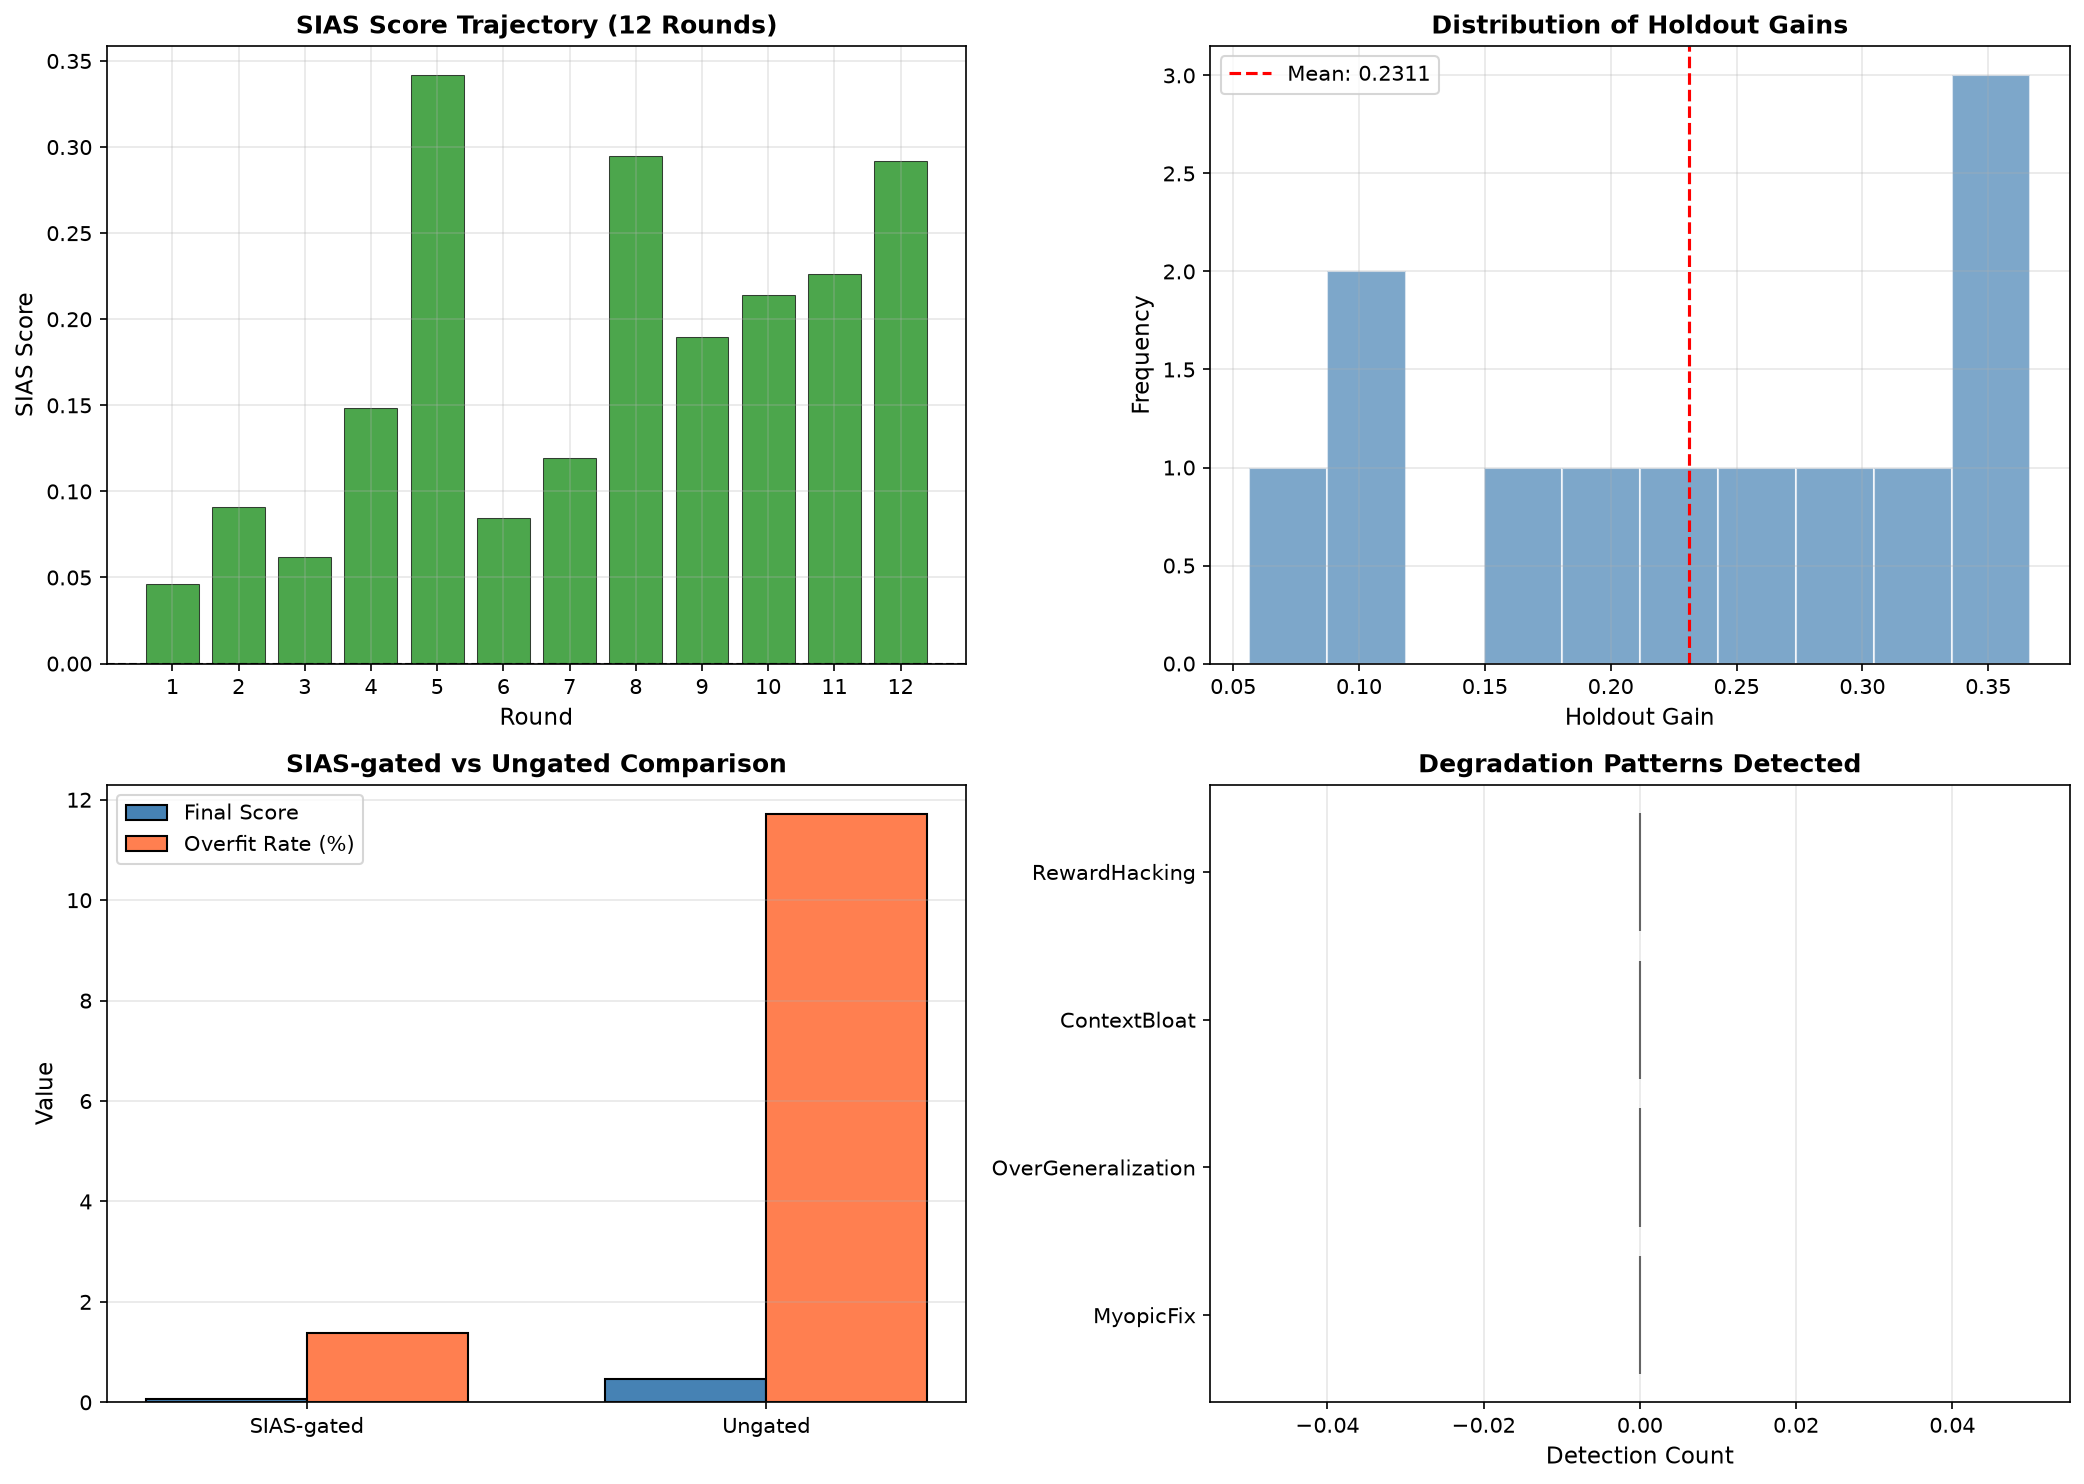
\includegraphics[width=0.9\textwidth]{figures_fig1_sias_trajectory.png}%
}{%
  \fbox{\parbox[c][5cm][c]{0.85\textwidth}{\centering [Figure 1 placeholder: figures\_fig1\_sias\_trajectory.png not found --- compile with the figure file in this directory, or use the `draft' class option.]}}%
}
\caption{SIAS score trajectory over 12 rounds of recursive improvement.}
\label{fig:trajectory}
\end{figure}

\begin{figure}[h]
\centering
\IfFileExists{figures_fig2_ablation.png}{%
  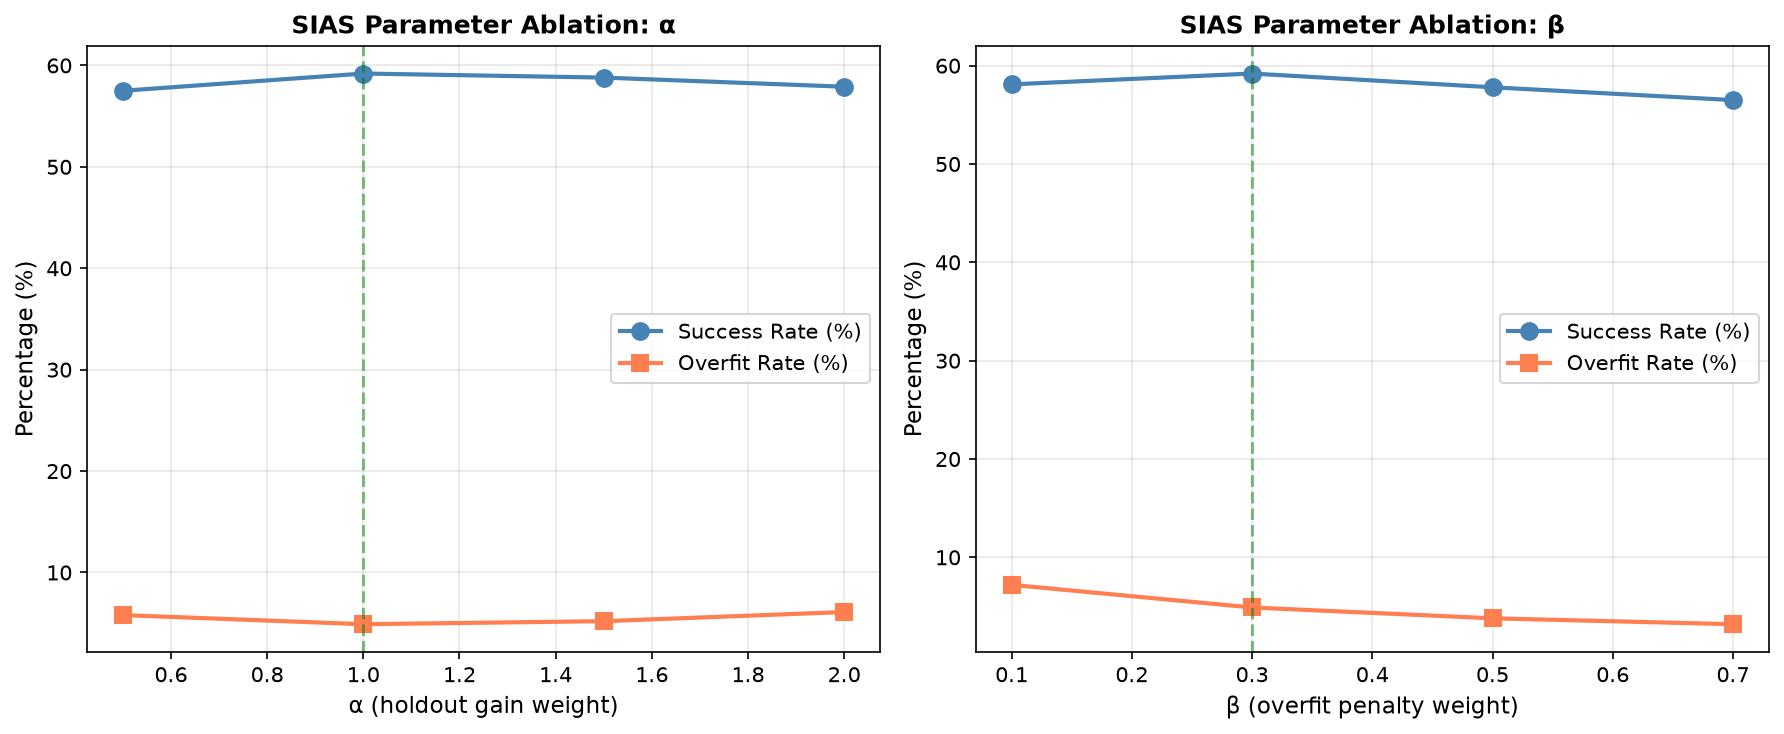
\includegraphics[width=0.9\textwidth]{figures_fig2_ablation.png}%
}{%
  \fbox{\parbox[c][5cm][c]{0.85\textwidth}{\centering [Figure 2 placeholder: figures\_fig2\_ablation.png not found --- compile with the figure file in this directory, or use the `draft' class option.]}}%
}
\caption{Parameter ablation for $\alpha$ and $\beta$.}
\label{fig:ablation}
\end{figure}

\section{Conclusion}
\label{sec:conclusion}

We presented SIAS and AI4AI-Bench for auditing recursive self-improvement in LLM agents. Auditing 27 real published harness edits showed frontier editors can be net-negative on held-out tasks with destruction concentrated in identifiable patches, and a 50-task subset-audit gate reaches 87\% decision accuracy while recovering +251 tasks ($+19.8$pp) relative to indiscriminate acceptance. Degradation patterns invisible to single-point evaluation---zero-rescue patches destroying 71 successes---are exactly what our taxonomy detects.

\bibliographystyle{plainnat}
\bibliography{references}

\end{document}
